% Workshop draft — §5.2. Independent of intro / §5.1 wording.
% Numbers: output/panocrowd_body_energy/metrics.json (PanoCrowd val∪test).

\section{Semantic Protection Is Content-Conditioned on Body Cuts}
\label{sec:body-boundary}

Class-weighted energy is the obvious semantic correction to ERP seam
carving: raise the cost of people so vertical seams take corridors
instead. Whether that term has work to do depends on whether the
spherical baseline already misses people. We test that with a
\emph{second} experiment, not as a replacement for the $2^\circ$ head-disk
measurement of~\S\ref{sec:head-disks} (head-point disks as energy and
metric). After that head-disk run, scoring the same spherical seams
against a larger body-column proxy left the baseline hit rate in an
unsettled band ($12.6\%$ mean, inside a pre-registered $[10\%,20\%)$
do-not-settle interval). Body-column energy versus spherical energy,
with body-column hits as the metric, was then locked as its own
experiment. It was not the original plan.

\paragraph{Protocol.}
PanoCrowd official val$\cup$test ($n=313$), not train. Density bins follow
the dataset's own counts; the claim bin is medium ($50$--$199$ heads,
$n=171$). Both configs use cyclic $8$-connected DP, $24$ seams at width
$\le 512$, $\lambda_g=\lambda_p=1$. Config (b) is gradient$\times\cos\phi$
only ($\lambda_s=0$). Config (c) adds semantic energy ($\lambda_s=4$) from
GT head points painted as body columns: a meridian strip from each head
downward by $12^\circ$ of latitude, half-width $2.5\times$ the
latitude-aware $2^\circ$ head radius. A person is hit if any of the first
$k$ original-width seams cuts that column. Primary $k=24$. We also
record $k\in\{8,48\}$; $k=48$ is not the claim (at $k=8$ the high-body
effect below is already $-17.2$\,pp on $48/49$ images).

\paragraph{Pre-registered subset.}
High-body is locked from (b) \emph{before} (c): medium images whose
spherical baseline already hits at least $20\%$ of body columns
($n=49$). The threshold is the same $20\%$ used as the proxy-artifact
bar on the earlier body-scoring check; it does not depend on (c). The
complement is the rest of medium ($n=122$). The support bar, unchanged
from the head-disk experiment, is a mean reduction of at least $5$\,pp
and a majority of images with (c)$<$(b). Characterized-boundary requires
that bar on high-body and not on the complement. That is what makes the
subset a predicted split rather than a slice found after seeing (c).

\paragraph{Limitation (read with the high-body row).}
Body columns are a constructed proxy, not person masks. Near-field
columns still cover mostly head and shoulders; in dense crowds they
merge (image 729: $38\%$ equatorial cover). The high-body subset---the
row whose reduction is $-35.2$\,pp, $49/49$---is exactly where merging
is most likely, so some scored hits can include a neighbor. RGB overlays
on stems $149$, $219$, $166$, $151$, $157$, and $729$ show columns
landing on people, not on floor or sky; the proxy is therefore not a
veto. Direction and unanimity ($49/49$) are robust to it. The
\emph{magnitude} ($-35.2$\,pp versus some smaller true person-cut rate)
carries proxy uncertainty and is not an exact body-IoU.

\begin{figure}[t]
  \centering
  \begin{minipage}[t]{0.32\linewidth}
    \centering
    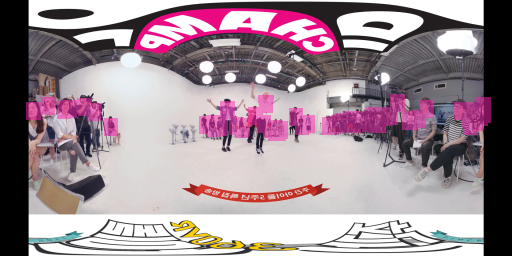
\includegraphics[width=\linewidth]{figures/fig_body_166.png}\\
    {\small 166 (medium, spaced)}
  \end{minipage}\hfill
  \begin{minipage}[t]{0.32\linewidth}
    \centering
    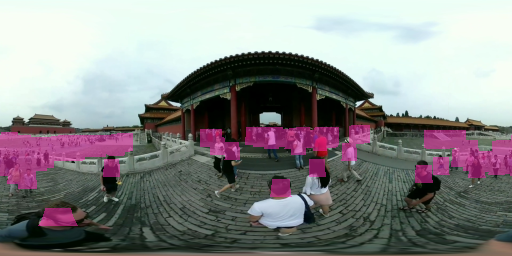
\includegraphics[width=\linewidth]{figures/fig_body_149.png}\\
    {\small 149 (medium, overlap)}
  \end{minipage}\hfill
  \begin{minipage}[t]{0.32\linewidth}
    \centering
    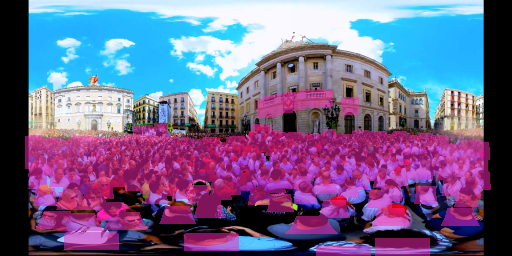
\includegraphics[width=\linewidth]{figures/fig_body_729.png}\\
    {\small 729 (dense, 38\% cover)}
  \end{minipage}
  \caption{Body-column proxy on RGB (magenta). Columns land on people,
  not floor or sky. Near-field boxes are still mostly head/shoulders;
  dense crowds merge. The high-body subset is the regime where merging
  is most likely, which bounds the $-35.2$\,pp magnitude.}
  \label{fig:body-proxy}
\end{figure}

\begin{table}[t]
\centering
\caption{Body-column hit rates, $k=24$. High-body: medium and (b)
body-hit $\ge 20\%$, locked from (b) only. Head-disk rates are a
separate experiment (\S\ref{sec:head-disks}) and are not in this table.}
\label{tab:body-boundary}
\begin{tabular}{lrrrrr}
\toprule
Set & $n$ & hit (b) & hit (c) & $\Delta$ & (c)$<$(b) \\
\midrule
High-body (locked) & $49$ & $35.4\%$ & $0.2\%$ & $-35.2$\,pp & $49/49$ \\
Medium complement & $122$ & $3.4\%$ & $0.0\%$ & $-3.4$\,pp & $77/122$ \\
All medium (tail-pulled) & $171$ & $12.6\%$ & $0.1\%$ & $-12.5$\,pp & $126/171$ \\
\bottomrule
\end{tabular}
\end{table}

\paragraph{The boundary is the pair.}
On high-body, (c) drives hits from $35.4\%$ to $0.2\%$
($-35.2$\,pp), every image. On the complement, (b) already hits only
$3.4\%$ of columns; (c) uses that entire ceiling ($-3.4$\,pp) and misses
the $5$\,pp bar. The all-medium $-12.5$\,pp mean is the $49$-image tail:
it is not an unconditional medium-bin win, which is why the subset was
locked first. Semantic energy does essentially all it can in both rows;
the rows differ in how much there was to do.

\begin{figure}[t]
  \centering
  \begin{minipage}[t]{0.48\linewidth}
    \centering
    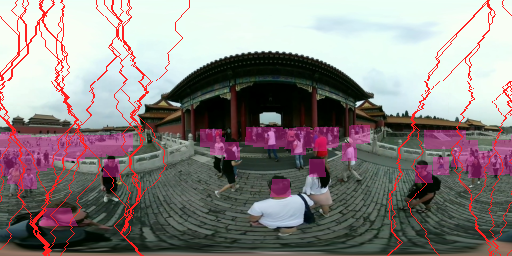
\includegraphics[width=\linewidth]{figures/fig_body_seams_b.png}\\
    {\small (b) spherical seams}
  \end{minipage}\hfill
  \begin{minipage}[t]{0.48\linewidth}
    \centering
    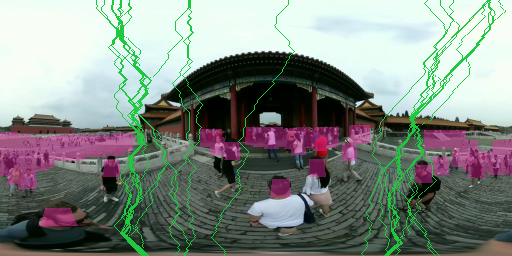
\includegraphics[width=\linewidth]{figures/fig_body_seams_c.png}\\
    {\small (c) body-column energy}
  \end{minipage}
  \caption{Largest high-body protection example. Magenta: body columns.
  Red: (b) seams that still cut people. Green: (c) seams after
  $\lambda_s=4$. Illustration of the $49/49$ direction, not a mask-quality
  claim.}
  \label{fig:body-seams}
\end{figure}

Semantic seam protection is content-conditioned: near-perfect on the
subset where the spherical baseline already cuts body columns, redundant
where it does not.

\subsection{A Content-Conditioned Rule}
\label{sec:content-rule}

The pair of rows supports a decision rule on an existing energy term.
Run the spherical baseline (b). Apply the semantic term (c) \emph{only}
on images where (b)'s seams cut protected body columns above a
threshold; skip it elsewhere. Motivation is the split already in
Table~\ref{tab:body-boundary}: protection is near-total where the
baseline cuts bodies, and redundant where it does not, so unconditional
$(c)$ spends compute---and risks over-smoothing---on the $\sim 72\%$ of
medium images ($122/171$) that do not need it. This is a reframing of
C2b, not a new experiment. $k=24$ remains primary; $k=48$ is not the
claim.

\paragraph{Oracle gate (upper bound).}
High-body in C2b is defined from ground-truth head points painted as
constructed body columns, locked from (b) before (c). The
$-35.2$\,pp / $-3.4$\,pp split is therefore the rule's
\emph{oracle bound}: performance when the gate knows where bodies are.
It is not a deployable score.

\paragraph{Practical gate (not evaluated).}
At inference there is no GT. The detector would be the segmenter's own
prediction of the same columns, then the same (b)-hit threshold. That
practical gate is motivated by the oracle split and has not been run.
We do not report $-35.2$\,pp as the performance of a GT-free method.

The rule adds a conditional to $\lambda_s$. It is a gating heuristic,
not a new retargeting paradigm and not a new algorithm class.

